\documentclass[11pt]{article}
\usepackage[margin=0.85in]{geometry}
\usepackage{amsmath,amssymb,amsthm,booktabs,longtable,array,graphicx,microtype}
\usepackage{xcolor,tikz,pgfplots,caption,float}
\pgfplotsset{compat=1.18}
\setlength{\emergencystretch}{2em}
\usepackage[breaklinks=true,colorlinks=true,linkcolor=blue,urlcolor=blue,citecolor=blue]{hyperref}
\newtheorem{theorem}{Theorem}
\newtheorem{lemma}[theorem]{Lemma}
\newtheorem{proposition}[theorem]{Proposition}
\newtheorem{corollary}[theorem]{Corollary}
\theoremstyle{definition}\newtheorem{definition}[theorem]{Definition}
\newcommand{\E}{\mathbb E}\newcommand{\R}{\mathcal R}
\title{A Conditional Stochastic Optimization of the Minish Cap Figurine Gallery\\and Distillation into Observable Human Policies}
\author{Project lead and curator: jciardullo\\\small Human-directed, AI-assisted computational research}
\date{8 October 2026\\[0.4em]\small Version 1.0}
\begin{document}\maketitle
\begin{abstract}
\emergencystretch=2em
We minimize expected gallery-attributable completion time for all 136 figurines, allowing every legal integer wager, capped resources, progressive eligibility, and discrete acquisition. For the conditional frozen reference inputs, the nominal model gives approximately 119.41 minutes (PAL/European) and 112.78 minutes (NTSC-U). These numbers are not certified whole-game route optima or microsecond-accurate measurements. The separate policy-distillation problem seeks the best tested memorable strategy under an explicit complexity budget. Its memorized option is the predeclared empirical regional Pareto knee; a 5\% worst-tested regret is a target, not an admissibility restriction.
The memorized knee options take 130.11 minutes (PAL) and 122.53 minutes (US) on the reference route; worst-tested regrets are 22.78\% and 21.10\%. The recommended one-page compact tables reduce worst regret to 8.14\% and 7.56\%. No human policy assessed by deterministic forward occupancy evaluation in the original bounded set or these supplemental audits attained the future-informed 5\% diagnostic. The supplemental US endpoint reaches 7.47\% at $C=39$; the lower-complexity original compact remains recommended.
\end{abstract}

\clearpage
\section*{Player Result: recommended one-page strategy}
\noindent\fbox{\begin{minipage}{.94\linewidth}\small
\textbf{Use the compact table if you can keep one small reference handy.} The knee remains the memorized option, not the default table recommendation. Collect completionist rewards normally; use ordinary town visits rather than special early detours.

\textbf{Read chance at the default one-shell wager.} All chance conditions below refer to that displayed percentage. ``Greater than'' excludes equality; ``at least'' includes equality. Fortress means completed Fortress of Winds; Water and Wind mean the respective Elements acquired. Before full eligibility, start a session only at \textbf{PAL: at least 700 shells and default displayed chance at least 20\%}, or \textbf{NTSC-U: at least 800 shells and default displayed chance at least 20\%}. In either region, held shells must also be strictly greater than the current row's reserve. Once started, keep using the current row even if chance drops below 20\%. Stop when shells are at or below the reserve. A pull may take you below it.
\begin{center}\begin{tabular}{@{}>{\raggedright\arraybackslash}p{.25\linewidth}>{\raggedright\arraybackslash}p{.345\linewidth}>{\raggedright\arraybackslash}p{.345\linewidth}@{}}\toprule
Phase & PAL reserve / wager & NTSC-U reserve / wager\\\midrule
Before Fortress & 600 / Wager 1 shell if default one-shell chance is greater than 80\%; otherwise raise display to 100\%. & 600 / Wager 1 shell if default one-shell chance is greater than 80\%; otherwise raise display to 100\%.\\
Fortress $\to$ Water & 150 / Raise display to 100\%. & 100 / Raise display to 100\%.\\
Water $\to$ Wind & 800 / Raise display to 100\%. & 800 / Raise display to 100\%.\\
Wind $\to$ full eligibility & 0 / Wager 1 shell if default one-shell chance is greater than 15\%; otherwise raise display to 100\%. & 0 / Wager 1 shell if default one-shell chance is greater than 20\%; otherwise raise display to 100\%.\\
Full eligibility & 0 / Wager 1 shell if default one-shell chance is greater than 8\%; otherwise raise display to 100\%. & 0 / Wager 1 shell if default one-shell chance is greater than 9\%; otherwise raise display to 100\%.\\
\bottomrule\end{tabular}\end{center}
\textbf{Short of the prescribed wager?} Bet all held shells. Never farm/buy during an early session. After full eligibility, restock when empty: buy as many already-funded bundles as possible, up to three PAL or four US. If none are affordable, farm only the missing money to fund the full batch: 900 R PAL or 800 R US. Purchases must fit below 999 shells.

\textbf{What does full eligibility mean?} Finish the ending, then the remaining completionist progression, sidequests, exploration, and Kinstone rewards that can unlock figurines, excluding rewards that themselves require gallery completion. The ending alone is insufficient; while those tasks remain unfinished, use the story rows. This conservative completionist milestone needs no chest-order knowledge, but the machine does not provide a separate ``all 136 eligible'' indicator.

\textbf{Near 999 shells?} Use an ordinary visit when the entry test is met; otherwise continue progression. Some overflow is accepted. Reference times: 122.04 min PAL and 115.29 min US; worst-tested regret: 8.14\% and 7.56\%. Neither meets 5\%. Fast text/B held and the paper's conditional resource/timing assumptions apply.
\end{minipage}}
\clearpage

\section{Problem Definition}
The completionist standard includes permanent/item upgrades, Pieces of Heart, every Kinstone fusion and its unlocked reward, all figurines, equippable inventory, Tiger Scrolls, and four Elements. The equippable category comprises the sword progression through Four Sword, bombs/Remote Bombs, bow/Light Arrows, boomerang/Magical Boomerang, shield/Mirror Shield, lantern, Gust Jar, Cane of Pacci, Mole Mitts, Roc's Cape, Pegasus Boots, Ocarina, and four bottles; unused items and transient contents are excluded.
Ordinary progression, encountered completionist collection, and ordinary town access contribute zero additional gallery time. Deliberate pulls and deliberate farming/shop cycles contribute time. This is not optimization of the entire movement route.
\begin{definition}
The full nominal state records the frozen event, owned figurines, shells, gallery cash, wallet capacity, and any required deliberate acquisition location. The mathematical optimizer may use the complete frozen future sequence. A human rule observes only the displayed one-shell new-figurine chance, held shells, cash, wallet, version, recognizable story milestones, and whether full eligibility has been reached. It cannot query future pickups, a route event index, an owned-count lookup, or hidden RNG state. Full eligibility is a completionist condition, not a flag displayed by the machine; the player-facing interpretation is given in the Player Result below.
\end{definition}
\section{Verified Game Mechanics}
For eligible count $U$ and owned count $F<U$,
\[
 b(F,U)=\max\{1,\lfloor100(U-F)/U\rfloor\},\quad
 1\le s\le\min\{S,101-b\}.
\]
The nominal actual success probability is
\[
 p(F,U,s)=\frac{\max\{h(F),b+s-1\}}{100},\qquad
 h(F)=\begin{cases}15&F<50,\\12&50\le F<80,\\9&80\le F<110,\\6&110\le F<136.\end{cases}
\]
A success adds one eligible unowned figurine; a failure adds no figure and pays 5 capped rupees. Figure identity selection is not uniform. EU and US eligibility is verified independently in the pinned decompilation, rather than inferred by scaling times. Productive pulls are unavailable when $F=U$. See the source audit and primary-source files~\cite{device,eligibility,prices,caps}.
\section{Resource Model}
The conditional reconstruction contains 3591 guaranteed shells, including 120 from six Cucco rewards, across 46 source records. Four fusion-chest amounts rely on source comments because active binary chest data are unavailable. First-encounter assignments and optional prerequisites are conditional route inputs; this is not an exhaustive independently certified 100\% itinerary.
For every encountered shell event $g$, received $=g$, retained $=\min(g,999-S)$, and overflow $=g-\min(g,999-S)$. Purchased shells are never knowingly discarded.
PAL bundles cost 300 R for 30 shells; NTSC-U bundles cost 200 R. Each sequential transaction requires cash and $S+30\le999$. There are at most three PAL or four US bundles per visit. Farming pickups apply $R\leftarrow\min(W,R+20)$; refunds apply $R\leftarrow\min(W,R+5)$. No unrelated naturally obtained rupees or random drops are credited. The house farm requires Mole Mitts.
\section{Timing Model}
The selector resets to one shell before each wager-selection stage: the pinned device source assigns \texttt{shells = 1} on entry and again when the next selection opens (lines 122 and 247)~\cite{device}. Thus every entry-cost calculation starts at 1. Fast text speed and holding B are assumed. PAL timing is $t(s)=20+(s-1)/15$ seconds. NTSC timing is $20+d(1,s)/15$, where $d$ is the shortest path on the legal clamped $\pm1,\pm10$ graph. Equal physical duration of these inputs is empirical.
A restocking cycle from Carlov costs 45 seconds travel if farming is needed and 20 seconds if already funded, plus 15 seconds per bundle. Each 20-R pickup costs $1200/r$ seconds at rate $r$ R/min. A genuine farm-area entry omits the outbound 20-second leg. All frozen main scenarios begin deliberate cycles at Carlov.
\section{State Space and Bellman Equation}
The nominal finite stochastic shortest-path problem has terminal condition $V=0$ at $F=136$ and equation
\[
 V(x)=\min_{a\in A(x)}\left(c(x,a)+\sum_y P(y\mid x,a)V(y)\right).
\]
The wager branch is
\[
 Q_s=t(s)+pV(e,F+1,S-s,R)+(1-p)V(e,F,S-s,\min(W,R+5)).
\]
Progression immediately applies the next frozen event and its receipts. A macro acquisition action includes a reachable number of discrete farming pickups and sequential purchases, preserving excess cash. The farming suffix envelope considers all reachable counts until the cap; it does not impose minimum funding or exhaust-natural-first heuristics. Locations are collapsed only through the documented macro travel costs. For a compact early visit, the internal activation test checks the regional entry thresholds, and the pull selector immediately stops at or below the phase reserve. Requiring shells above that reserve in the player-facing entry wording therefore removes only zero-pull sessions; it leaves wagers and modeled time unchanged.
\section{State Reductions}
\begin{lemma}[Nested eligibility]
If each eligible set is contained in every later eligible set, success adds exactly one new eligible identity, and nominal success depends only on $F,U,s$, then owned identity may be replaced by count without changing nominal transition probabilities or attainable values.
\end{lemma}
\begin{proof}
Every owned identity remains eligible. Thus the number of unowned eligible identities is exactly $U-F$. Success and duplicate outcomes preserve the same count/resource transition for every owned set of size $F$. Induction across nested unlocks gives a count-state Markov model. Nonuniform successful identity selection does not affect this argument. Without nested sets the reduction is invalid.
\end{proof}
\begin{lemma}[Exact cash compression]
Starting at zero, cash under $+5$ refunds, $+20$ farming, regional purchases, and the modeled wallet caps $\{300,999\}$ lies in residues 0 or 4 modulo 5.
\end{lemma}
\begin{proof}
All uncapped increments and costs preserve residue. The only ordinary cap in the frozen state inputs is 300, congruent to 0 modulo 5; the 999 cap contributes residue 4. No other wallet capacity occurs in these route inputs. These residues are closed under all subsequent operations. The 400 represented cash values are therefore an exact reachable superset, not rounded balances.
\end{proof}
Supplemental outside cash is introduced explicitly and tested separately; it does not retroactively change the zero-cash theorem.
\section{Lemmas and Propositions}
\begin{proposition}[Resource conservation]
For every completed run,
\[
 S_{\rm natural,ret}+S_{\rm purchased}=S_{\rm consumed}+S_{\rm end},
\]
\[
 R_{\rm refund,ret}+R_{\rm farm,ret}+R_{\rm external,ret}
 =R_{\rm purchases}+R_{\rm end}.
\]
\end{proposition}
\begin{proof}
Sum each exact receipt, wager, refund, farming, and transaction change. Caps remove only the separately recorded overflow quantities. Intermediate terms telescope.
\end{proof}
\begin{proposition}[Wager entry]
Breadth-first search on the directed legal input graph gives the minimal number of adjustment inputs. A 20-shell target takes three inputs via $1\to11\to21\to20$ when 21 is legal, or two via a clamp when the limit is 20.
\end{proposition}
\begin{proof}
Every edge represents one permitted physical input with its actual clamp. BFS enumerates paths in nondecreasing edge count; first arrival minimizes that count.
\end{proof}
\begin{lemma}[Uniform expected macro-decision bound]
In the finite nominal model, every policy induced by the legal macro action set is proper and has at most
\[
 \begin{aligned}N_{\max}&=\frac{50}{.15}+\frac{30}{.12}+\frac{30}{.09}+\frac{26}{.06}=1350,\\
 H&=N_{\max}+\frac{100N_{\max}+999}{30}+8=5891.3.\end{aligned}
\]
expected macro decisions from any valid route/resource state.
\end{lemma}
\begin{proof}
There is no idle, abort, or farm-only action. Progression can occur at most eight times; after the last event, waiting is illegal. With finitely many pulls, only finitely many purchases are possible because purchases strictly increase shells, which are capped, and purchased shells cannot be discarded. Thus a nonterminating path must contain infinitely many productive pulls. At each count the conditional success hazard is at least the applicable hidden floor; the probability of $k$ consecutive failures is at most $(1-h/100)^k$. Hence the next success occurs almost surely, and induction over the remaining counts proves that every legal policy reaches $F=136$ almost surely (properness).
Summing reciprocal lower hazards bounds expected productive pulls by $N_{\max}=1350$, including adaptive wagers. Every wager consumes at most 100 shells. For each finite path prefix, conservation bounds restocking trips by $(100N_{\rm pulls}+999)/30$, since every trip buys at least 30 shells and retained natural receipts are nonnegative. Monotone convergence and the pull bound give the stated uniform expected macro-decision bound. This applies from every valid state, not only to policies assumed in advance to complete.
\end{proof}
\section{Main Optimality Theorem}
\begin{proposition}[Existence and uniqueness in the conditional nominal model]
For either regional finite macro model, the optimal value is the unique finite Bellman solution, and a deterministic stationary minimizing selector attains it.
\end{proposition}
\begin{proof}
Let $\tau$ be the number of macro decisions before termination. The preceding lemma establishes $\sup_\pi\E_x^\pi\tau\le H$ uniformly in valid $x$, for every policy induced by the legal action set. For bounded functions $V,W$ vanishing on terminal states, the finite-horizon dynamic-programming representation and the inequality for minima imply
\[
 \|T^n V-T^n W\|_\infty
 \le \sup_{x,\pi}\Pr_x^\pi(\tau>n)\,\|V-W\|_\infty
 \le \frac{H}{n}\|V-W\|_\infty.
\]
For integer $n>2H$, the contraction factor is strictly below $1/2$. The unique fixed point of $T^n$ is also fixed by $T$, since the iterates commute and $T$ maps that fixed point to another fixed point of $T^n$. A minimizing stationary selector exists because action sets are finite. Properness and finite expected termination permit telescoping its Bellman equality, so its value equals the fixed point. The Bellman inequalities give the corresponding lower bound for every other legal policy.
\end{proof}

\begin{theorem}[Conditional Bellman certificate]
Assume verified nominal mechanics, the frozen regional resource sequence, stated timing parameters, legal macro actions, and a uniformly bounded Bellman residual $\|\widehat V-T\widehat V\|_\infty\le\epsilon$, including arithmetic error, with zero terminal value. Then
\[
 |\widehat V(x_0)-V^\star(x_0)|\le H\epsilon.
\]
\end{theorem}
\begin{proof}
For every legal action, the Bellman residual gives $\widehat V(x)\le c(x,a)+P_a\widehat V(x)+\epsilon$. Telescope along an optimal policy to obtain $\widehat V(x_0)\le V^\star(x_0)+\epsilon\E\tau$. Along a minimizing selector, the reverse inequality yields $V^\star(x_0)\le\widehat V(x_0)+\epsilon\E\tau$. Apply the expected-decision bound.
\end{proof}

\begin{corollary}[PAL reference problem]
Assume the frozen European reference event sequence, nested eligibility, nominal success law above, capped shells/cash, 300-R bundles with a three-bundle limit, PAL entry time, and stated macro travel/farming costs. Then the unique optimal Bellman solution satisfies
\[
 V_{\rm PAL}(x_0)=T^\star_{\rm PAL}:=\inf_\pi\E_{\rm PAL}^{\pi}[T_{\rm gallery}].
\]
\end{corollary}
\begin{proof}Apply the existence/uniqueness proposition to this regional action and transition model.\end{proof}
\begin{corollary}[NTSC-U reference problem]
Assume the separately frozen US eligibility/event sequence, nominal success law, caps, 200-R bundles with a four-bundle limit, legal-input shortest-path entry costs under equal input duration, and stated macro travel/farming costs. Then
\[
 V_{\rm US}(x_0)=T^\star_{\rm US}:=\inf_\pi\E_{\rm US}^{\pi}[T_{\rm gallery}].
\]
\end{corollary}
\begin{proof}Apply the same proposition to the independently constructed US model; it is not a rescaling of the European model.\end{proof}

At $10^{-6}$ and $10^{-7}$ seconds of \emph{certified uniform residual}, these bounds would be below 0.0058913 and 0.00058913 seconds. Reported floating-point residuals alone do not establish those rigorous intervals. The regional computations give
\[
 \widehat V_{\rm PAL}(x_0)=7164.500603\ \mathrm{s},\qquad
 \widehat V_{\rm US}(x_0)=6766.617683\ \mathrm{s}.
\]
These are conditional numerical optimality results. This paper does not claim a directed-rounding proof of the displayed digits, an exact full-playthrough PRNG optimum, or an unconditional whole-game optimum.
\section{Computer-Assisted Optimization and Numerical Validation}
Policy iteration evaluates functional same-count transition graphs and improves over every legal integer wager and reachable acquisition action. Independent forward occupancy evaluation verifies expectations, terminal mass, and resource conservation. A smaller exhaustive-action model agrees with linear programming and value iteration. The $10^{-7}$ repeat leaves reference selected policy tables unchanged; sampled tie sets can narrow. Pre-Mitts farming restrictions are re-solved or certified by feasibility of a selected policy attaining the relaxed initial lower bound.
Floating-point arithmetic error is assessed through independent evaluation and tighter solves; it is not rigorously bounded by interval arithmetic. Accordingly the residual theorem is mathematical, while the reported machine residuals and agreement are numerical evidence. Monte Carlo is validation, not proof of optimality.
\begin{table}[H]\centering\small
\begin{tabular}{ll}\toprule
Evidence & Scope\\\midrule
Residual target & $10^{-6}$ s; repeat $10^{-7}$ s\\
Expected macro bound & $H=5891.3$\\
Arithmetic certification & No directed-rounding bound established\\
Forward conservation & Shell/cash errors tested below $10^{-7}$\\
Policy stability & Reference selected tables unchanged on tightening\\
\bottomrule\end{tabular}
\caption{Numerical evidence and certification limits}\label{tab:result-1}\end{table}
The fresh validation comprises 960,000 completions across 48 cells. Deterministic cells can miss a zero-width confidence interval by floating-point summation alone; they are checked with a numerical tolerance instead. 
\section{Benchmark Corollaries}
\begin{corollary}[Conditional comparison]
Under identical frozen inputs and nominal costs, any feasible benchmark policy has expected time at least the model optimum. Restrictions to one shell, displayed 80\%, displayed 100\%, or a one-shell/guarantee threshold cannot improve the unrestricted action optimum.
\end{corollary}
\begin{proof}
These feasible action selections are contained in the unrestricted policy class.
\end{proof}
\begin{table}[H]\centering\small
\begin{tabular}{llrrrr}\toprule
Version & Policy & Minutes & Shells & Pulls & Trips\\\midrule
PAL & one & 173.67 & 521.0 & 521.0 & 0.00\\
PAL & guarantee & 254.80 & 7533.0 & 136.0 & 45.00\\
PAL & eighty & 218.34 & 6664.0 & 168.3 & 35.30\\
PAL & optimal & 119.41 & 3719.9 & 338.2 & 1.49\\
NTSC-U & one & 173.67 & 521.0 & 521.0 & 0.00\\
NTSC-U & guarantee & 194.56 & 7535.0 & 136.0 & 34.00\\
NTSC-U & eighty & 171.37 & 6667.3 & 168.3 & 26.79\\
NTSC-U & optimal & 112.78 & 3950.9 & 306.7 & 3.10\\
\bottomrule\end{tabular}
\caption{Reference benchmarks with full-route-knowledge progression/restocking}\label{tab:result-2}\end{table}

\begin{table}[H]\centering\small
\begin{tabular}{llrrrr}\toprule
Region & Threshold & Minutes & Shells & Pulls & Trips\\\midrule
PAL & 9 & 130.25 & 2334.7 & 346.5 & 4.42\\
PAL & 27 & 178.53 & 5420.6 & 206.2 & 24.00\\
NTSC-U & 10 & 123.35 & 2428.4 & 333.0 & 4.48\\
NTSC-U & 27 & 145.75 & 5420.6 & 206.1 & 18.02\\
\bottomrule\end{tabular}
\caption{Threshold benchmarks on the reference route with full-route-knowledge progression/restocking}\label{tab:result-3}\end{table}
Threshold benchmark progression/restocking is optimized with full route knowledge. Such a benchmark is not itself a complete observable player rule.
\section{Policy Distillation}
\begin{definition}[Best tested simplicity--performance curve]
Let $\Omega_v$ be the tested regional route/timing set. For observable human policy $\pi$,
\[
 R_v(\pi)=\max_{\omega\in\Omega_v}\frac{T_\pi(\omega)-T^\star(\omega)}{T^\star(\omega)},\quad
 R_v^\star(c)=\min_{\pi\in\Pi_{\rm tested},\ C_v(\pi)\le c} R_v(\pi).
\]
The minimum is over tested policies assessed by deterministic forward occupancy evaluation, not every conceivable simple strategy. Human-policy regret is measured against a scenario-specific optimizer that knows the frozen future resource sequence. It therefore combines policy-simplification loss with value-of-information loss and is not a comparison under matched information.
\end{definition}
Complexity is $C_v=4P_v+2S_v+Q_v+2I_v+L_v+2M_v+B_v$, counting distinct progression boundaries, shell thresholds, chance thresholds, intermediate values, clauses, session flags, and restocking branches. Regional differences $D$ are charged only in a combined guide. The full vector $(P,S,Q,I,L,M,D,B)$ is published. Here $P$ counts remembered progression boundaries, $S$ distinct inventory thresholds, $Q$ distinct displayed-chance thresholds, $I$ distinct intermediate wagers/targets, $L$ decision clauses, $M$ persistent session flags, $D$ explicit differences in a combined regional guide, and $B$ distinct restocking branches. Individual scores omit $D$ because a player learns only one version.
The normalized endpoint chord joins $(0,1)$ and $(1,0)$. Signed desirable improvement is $(1-\widetilde C-\widetilde R)/\sqrt2$. The largest positive interior improvement selects the knee; if none exists, choose the least-complex frontier policy. The 5\% target is not a filter.
A total of 10,000 frozen candidates covers universal thresholds, two-phase rules, cap pressure, chance/inventory bands, intermediate tables, and four recognizable story phases. Universal cuts sweep every integer 0--100; coarse-to-fine beam refinement uses nominal width 32, integer chance refinements, and ten-shell inventory increments. Tier 4 has at most eight printed clauses and four intermediate values. Generation, grids and deterministic candidate parameters are published.

The 512-run common-random-number signal is not a deterministic empirical dominance test. A fresh holdout seed 20261110 evaluates the frozen list; simultaneous approximate 99\% studentized intervals use critical value 5.582881.\footnote{For each fixed policy/case, studentize its sample mean completion time using $\widehat{\mathrm{SE}}=\sqrt{a^\top\widehat\Sigma a/512}$, where $\widehat\Sigma$ is the unbiased sample covariance of four trajectory cost components and $a$ is that case's cost vector. The two-sided Bonferroni cutoff is $t_{511}^{-1}(1-0.01/(2\cdot10{,}000\cdot26))=5.58288113636$. The family is all 260,000 frozen candidate/case means, covering both regions and all timing cases. Common indexed random draws remain shared across candidates; timing cases re-cost the same trajectories. Within-trajectory component covariance is retained. No cross-candidate covariance or paired-difference standard error is used, and Bonferroni does not require independence among these marginal intervals. Approximate Student-t/normal mean behavior, finite sample variance, and IID completions within each fixed case are assumed. The fixed model optimum converts time intervals to relative-regret intervals; taking maxima yields the screening worst-regret bounds.} Candidates whose lower regret bound remains compatible with a lower/equal-complexity deterministically evaluated feasible incumbent survive, plus protected complexity-band and tier leaders. The uncertainty pool exceeds 32. Adaptive generation used separate earlier samples. Screening intervals are approximate, not a coverage theorem for arbitrary heavy-tailed outputs.

Final deterministic forward occupancy evaluation covers 2,816 regional policy records, at least six policies in every tier per region. Records never receiving that evaluation are marked not retained after screening. Previously evaluated records remain eligible even if a later screening step would remove them. Only policies receiving deterministic forward evaluation may establish final empirical Pareto dominance. These calculations use floating-point arithmetic, not exact arithmetic or directed-rounding certification.
\begin{table}[H]\centering\small
\begin{tabular}{llrrrrr}\toprule
Region & Selection & ID & C & Ref. min & Mean R\% & Worst R\%\\\midrule
PAL & minimal & 500 & 7 & 269.90 & 131.05 & 184.36\\
PAL & knee & 6457 & 14 & 130.11 & 10.29 & 22.78\\
PAL & compact & 8911 & 40 & 122.04 & 3.41 & 8.14\\
PAL & audit baseline & 10000 & 8 & 173.67 & 47.10 & 64.21\\
NTSC-U & minimal & 500 & 7 & 205.26 & 87.02 & 124.72\\
NTSC-U & knee & 6098 & 14 & 122.53 & 10.30 & 21.10\\
NTSC-U & compact & 8560 & 37 & 115.29 & 3.72 & 7.56\\
NTSC-U & audit baseline & 10000 & 8 & 173.67 & 55.88 & 71.64\\
\bottomrule\end{tabular}
\caption{Original named selections and separate audit baseline, assessed by deterministic forward occupancy evaluation}\label{tab:result-4}\end{table}
\begin{table}[H]\centering\small
\begin{tabular}{lll}\toprule
Region & Selection & $(P,S,Q,I,L,M,D,B)$\\\midrule
PAL & minimal & (1, 0, 0, 0, 2, 0, 0, 1)\\
PAL & knee & (1, 0, 2, 0, 5, 1, 0, 1)\\
PAL & compact & (4, 4, 4, 0, 8, 1, 0, 2)\\
PAL & audit baseline & (1, 0, 0, 0, 3, 0, 0, 1)\\
NTSC-U & minimal & (1, 0, 0, 0, 2, 0, 0, 1)\\
NTSC-U & knee & (1, 0, 2, 0, 4, 1, 0, 2)\\
NTSC-U & compact & (4, 3, 3, 0, 8, 1, 0, 2)\\
NTSC-U & audit baseline & (1, 0, 0, 0, 3, 0, 0, 1)\\
\bottomrule\end{tabular}
\caption{Audited per-player complexity feature vectors}\label{tab:result-5}\end{table}
\paragraph{Targeted endpoint audit.}
The seemingly simpler rule ``wait for full eligibility, then always wager one shell'' was absent from the frozen list, not screened out. Its early and postgame clauses differ, giving $(P,S,Q,I,L,M,D,B)=(1,0,0,0,3,0,0,1)$ and $C=8$, versus the shared universal wager clause of ID 500 at $C=7$. Supplemental audit ID 10000 uses maximum-bundle restocking and was evaluated deterministically on the existing 26 cases: reference 173.67 minutes in each region, mean regret 47.10\% PAL / 55.88\% US, and worst regret 64.21\% / 71.64\%. It added the PAL $C=8$ frontier point and dominated the former $C=8$ and $C=9$ points; it is dominated in US. The subsequent exhaustive $C\le8$ audit finds minimum-needed restocking (ID 14203) about $6.8\times10^{-7}$ seconds faster in PAL. This sub-microsecond floating-point difference is below the evaluation tolerance and is not a certified or practically meaningful dominance claim; both are retained as an unresolved numerical near-tie. ID 500 remains the minimum-complexity endpoint. That endpoint-only audit left both chords and knee IDs 6457/6098 unchanged, including the bounded weight/duplicate checks. The later expanded US normalization is reported below; it also leaves both knee IDs unchanged. The original 10,000 candidates remain frozen; this is one explicitly separate audit policy, not a new search. Table~\ref{tab:result-2}'s future-informed one-shell benchmark also rounds to 173.67 minutes, but this numerical agreement does not equate the policies or their information sets. The supplemental rule loses 2592 natural shells to the cap and arrives at full eligibility with 999; its tiny nonzero expected purchases are retained in machine-readable results.

The best minimal rule is the lowest worst regret at the minimum observed complexity. No human policy assessed by deterministic forward occupancy evaluation in this bounded tested set, including the supplemental audit, attained 5\% worst-tested regret. The original compact selection minimizes worst regret among Tier-4-compatible policies in the frozen evaluated candidate family, not maximum complexity. The separate supplemental US improvement is reported below and is not adopted as the recommendation. The simplest 5\% selection minimizes complexity, then worst and mean regret; neither region has a qualifying policy. The fixed software-helper benchmark has worst-tested regret 6.44\% for PAL and 5.83\% for NTSC-U. It uses an owned-count lookup, so it is excluded from the human-policy frontier.

Complexity counts distinct concepts after eliminating inactive parameters and identical adjacent rules. The full-eligibility boundary is counted; empty-shell feasibility and pool exhaustion are not learned inventory thresholds. An entry gate, each decision row, a meaningful partial-wager fallback and one conditional restocking clause are counted in $L$. $M$ counts the one retained active-session flag; $B$ counts branches separately. This explicit convention is not a validated cognitive metric.
\begin{figure}[H]\centering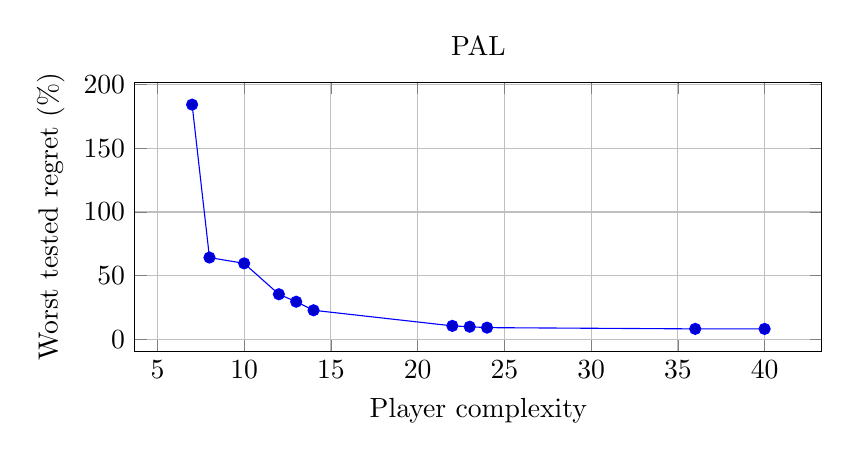
\begin{tikzpicture}\begin{axis}[width=.85\linewidth,height=5cm,xlabel={Player complexity},ylabel={Worst tested regret (\%)},title={PAL},grid=major]\addplot+[mark=*] coordinates {(7,184.362551) (8,64.214470) (10,59.629187) (12,35.366278) (13,29.500275) (14,22.782131) (22,10.536568) (23,9.865108) (24,9.145097) (36,8.167272) (40,8.136230)};\end{axis}\end{tikzpicture}\caption{PAL empirical frontier, including the minimal-policy endpoint.}\label{fig:frontier-1}\end{figure}
\begin{figure}[H]\centering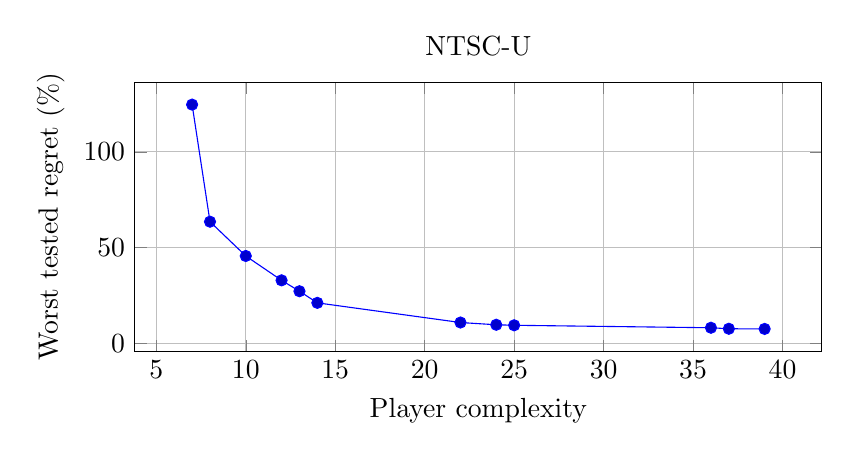
\begin{tikzpicture}\begin{axis}[width=.85\linewidth,height=5cm,xlabel={Player complexity},ylabel={Worst tested regret (\%)},title={NTSC-U},grid=major]\addplot+[mark=*] coordinates {(7,124.721733) (8,63.521589) (10,45.601097) (12,32.870613) (13,27.178619) (14,21.098848) (22,10.817411) (24,9.644194) (25,9.374940) (36,8.085787) (37,7.556752) (39,7.473862)};\end{axis}\end{tikzpicture}\caption{NTSC-U empirical frontier with the supplemental $C=39$ endpoint; the original compact at $C=37$ is retained.}\label{fig:frontier-2}\end{figure}

\begin{figure}[H]\centering
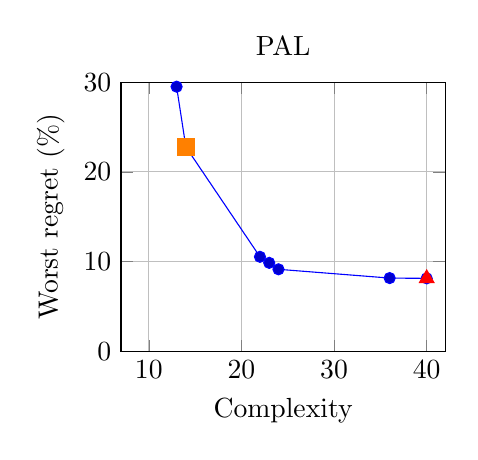
\begin{tikzpicture}\begin{axis}[width=.47\linewidth,height=5cm,ymin=0,ymax=30,xmin=7,xmax=42,xlabel={Complexity},ylabel={Worst regret (\%)},title={PAL},grid=major]\addplot+[mark=*] coordinates {(7,184.362551) (8,64.214470) (10,59.629187) (12,35.366278) (13,29.500275) (14,22.782131) (22,10.536568) (23,9.865108) (24,9.145097) (36,8.167272) (40,8.136230)};\addplot[only marks,mark=square*,orange,mark size=3pt] coordinates {(14,22.782131)};\addplot[only marks,mark=triangle*,red,mark size=3pt] coordinates {(40,8.13623)};\end{axis}\end{tikzpicture}
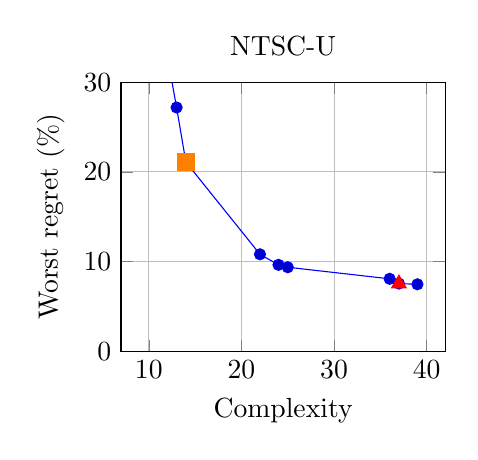
\begin{tikzpicture}\begin{axis}[width=.47\linewidth,height=5cm,ymin=0,ymax=30,xmin=7,xmax=42,xlabel={Complexity},ylabel={Worst regret (\%)},title={NTSC-U},grid=major]\addplot+[mark=*] coordinates {(7,124.721733) (8,63.521589) (10,45.601097) (12,32.870613) (13,27.178619) (14,21.098848) (22,10.817411) (24,9.644194) (25,9.374940) (36,8.085787) (37,7.556752) (39,7.473862)};\addplot[only marks,mark=square*,orange,mark size=3pt] coordinates {(14,21.098848)};\addplot[only marks,mark=triangle*,red,mark size=3pt] coordinates {(37,7.556752)};\end{axis}\end{tikzpicture}
\caption{Frontier detail at 0--30\% regret. Orange squares mark the memorized knees; red triangles mark the recommended compact-table options. Endpoint normalization uses the full frontier, not this cropped view. The supplemental US $C=39$ point is included; the red triangle remains the recommended historical compact.}\label{fig:frontier-detail}\end{figure}

% BEGIN SUPPLEMENTAL REVISION
\subsection{Knee-selection margins}
The historical frontier (including audit ID 10000) uses PAL endpoints $(C_{\min},C_{\max},R_{\max},R_{\min})=(7,40,1.843625511,0.081362298)$ and US $(7,37,1.247217326,0.075567517)$. Regrets here are fractions. The actual runner-up in both regions is ID 6729, not ID 10000. Full unrounded machine outputs accompany this paper.
\begin{table}[H]\centering\small
\begin{tabular}{llrrrr}\toprule
Region & ID & C & $\widetilde C$ & $\widetilde R$ & $d$\\\midrule
PAL & 6457 & 14 & 0.212121212 & 0.083108478 & 0.498347865\\
PAL & 6729 & 13 & 0.181818182 & 0.121230730 & 0.492818840\\
PAL & 3708 & 12 & 0.151515152 & 0.154517488 & 0.490709027\\
PAL & 10000 & 8 & 0.030303030 & 0.318217163 & 0.460665789\\
NTSC-U & 6098 & 14 & 0.233333333 & 0.115581428 & 0.460386787\\
NTSC-U & 6729 & 13 & 0.200000000 & 0.167472116 & 0.447264756\\
NTSC-U & 3708 & 12 & 0.166666667 & 0.216053137 & 0.436483013\\
US ext. & 6098 & 14 & 0.218750000 & 0.116206681 & 0.470256641\\
US ext. & 6729 & 13 & 0.187500000 & 0.168060683 & 0.455687411\\
US ext. & 3708 & 12 & 0.156250000 & 0.216607360 & 0.443456814\\
\bottomrule\end{tabular}
\caption{Historical and expanded knee scores near the maximum; ID 10000 included for context}\label{tab:knee-margins}\end{table}
Historical margins are 0.005529024706 PAL and 0.013122031146 US. The expanded US frontier changes its high-complexity endpoint to $(C_{\max},R_{\min})=(39,0.074738616523559787)$. Its knee/runner-up scores become 0.470256640980 / 0.455687410833, margin 0.014569230147; PAL is unchanged. Both knees remain selected. These nonzero geometric margins coexist with the bounded sensitivity result: two of sixteen weight/duplicate perturbations change each regional knee, also after the supplemental extension. A geometric margin does not remove dependence on the chosen complexity weights.
\subsection{Supplemental low-complexity grammar audit}
The machine-readable grammar is the interpreter in \texttt{policy.hpp}: one early row, a Fortress/Water/Wind split, or four story rows; each row has an inclusive shell/chance entry gate, reserve stop, strict chance threshold and displayed-target or fixed-shell action. Three postgame inventory bands share the same action form. The active flag persists only within a visit. An unaffordable early wager either ends the visit or spends all shells; postgame shortage instead invokes the chosen maximum-batch, minimum-needed, or already-affordable-first restocking rule. Version branches are only the verified price, batch limit and timing. No event, future-resource, owned-count or RNG input is introduced.
The canonical legal domains are shell gates/reserves 1--1000/0--999, chance thresholds 0--100, displayed targets 1--100, fixed wagers 1--100 (negative encoding), and the three restocking modes. Boundary aliases, inactive fields, identical adjacent rows, absent bands, one-shell aliases and probability-cap aliases are quotiented before evaluation. The C++ parser accepts redundant arbitrary integers; this audit concerns canonical legal behavior, not infinitely many serialized aliases. The complete grammar, domains, normalization and scripts are published in \texttt{supplemental/grammar.json}.
Every minimum-scored representative has $P\ge1$, $L\ge2$, $B\ge1$, hence $C\ge7$. Through $C=8$, inventory thresholds, intermediate values, extra progression boundaries and session gates cannot fit. The exhaustive partition is four $C=7$ classes; at $C=8$, 198 shared-chance-threshold classes, four different constant early/postgame rules, four no-early rules, two meaningful partial-guarantee rules, and two funded-first universal rules. All 214 canonical templates are valid and distinct; no template is rejected. Their 428 regional records evaluate every applicable route/timing case. Counts exclude redundant raw aliases analytically rather than sampling them.
At $C=15$, let $g$ be the early-session shell entry trigger and $r$ its stop reserve. The domains are $3\le g\le999$ and $1\le r\le g-2$, giving 497,503 inventory pairs. The factor eight comprises two early constant wagers (1 shell or displayed 100\%), two postgame constants (the same choices), and two restocking modes (maximum batch or minimum needed). This restricted subfamily contains
\[
 8\sum_{g=3}^{999}(g-2)=3{,}980{,}024
\]
distinct policies, each with vector $(1,2,0,0,4,1,0,1)$. Thus full enumeration through 15 is infeasible within this local revision. The highest genuinely exhaustive boundary is 8; results above it remain non-exhaustive. No heuristic search is substituted for the requested exhaustive audit. Original evaluated records through 15 number 217 PAL and 165 US; these supplement, rather than complete, the higher-complexity coverage.
\begin{table}[H]\centering\small
\begin{tabular}{llrr}\toprule
Region & ID & C & Worst R\%\\\midrule
PAL & 500 & 7 & 184.362551\\
PAL & 14203 & 8 & 64.214470\\
PAL & 4148 & 10 & 59.629187\\
PAL & 3708 & 12 & 35.366278\\
PAL & 6729 & 13 & 29.500275\\
PAL & 6457 & 14 & 22.782131\\
NTSC-U & 500 & 7 & 124.721733\\
NTSC-U & 75 & 8 & 63.521589\\
NTSC-U & 4124 & 10 & 45.601097\\
NTSC-U & 3708 & 12 & 32.870613\\
NTSC-U & 6729 & 13 & 27.178619\\
NTSC-U & 6098 & 14 & 21.098848\\
\bottomrule\end{tabular}
\caption{Supplemental combined low-complexity frontier; exhaustive only through 8, bounded tested results at 9--15}\label{tab:low-frontier}\end{table}
At PAL $C=8$, ID 14203 is the mechanically ordered frontier representative, while ID 10000 remains the named audit baseline. Their expected times differ by less than $10^{-6}$ seconds and are treated as an unresolved numerical near-tie.
Audit baseline ID 10000 waits for full eligibility, then always wagers one shell. At shortage it buys the maximum permitted batch: three PAL bundles (90 shells, 900 R) or four US bundles (120 shells, 800 R), farming missing money even if some bundles are already funded; a fully funded purchase uses direct-shop travel. Wallet and shell caps remain enforced. Its reference time is 173.67 minutes in each region, with compact savings 51.63/58.38 minutes and worst-tested regret 64.21\%/71.64\%. The reference time alone does not establish route robustness; this observable baseline is distinct from Table~\ref{tab:result-2}'s future-informed one-shell benchmark.
ID 500 remains the minimum endpoint; no original frozen frontier point is newly dominated. ID 10000 and minimum-needed ID 14203 differ below a microsecond and are treated as an uncertified numerical near-tie, even though the mechanical floating-point frontier orders them. The supplemental audit does not change either knee or any historical named selection.
\subsection{Local mutation neighborhood around the compact policies}
Before evaluation, the extension was limited to 12 printed clauses, four intermediate values (displayed 40/60/80 or fixed 30), and the current observable interface. It generates 40 single-row/one-inventory-band variants of each regional compact seed, without adaptive screening. After inactive-target/behavior normalization, 31 unique policies per region remain; zero are invalid. All 62 regional records receive deterministic evaluation. This is a local bounded mutation study, not an exhaustive search of the expanded grammar. Generated rules actually use at most nine clauses; both winning mutations still fit the original eight-clause Tier-4 limit.
\begin{table}[H]\centering\small
\begin{tabular}{llrrrr}\toprule
Region & ID & C & Worst R\% & Gain pp & Ref. saved s\\\midrule
PAL & 12003 & 42 & 8.145581 & -0.009352 & -0.679186\\
NTSC-U & 13011 & 39 & 7.473862 & 0.082890 & 8.020254\\
\bottomrule\end{tabular}
\caption{Best supplemental mutation versus the original regional compact; negative gain means worse}\label{tab:tier5}\end{table}
PAL ID 12003 has vector $(4,4,4,1,8,1,0,2)$; US ID 13011 has $(4,3,3,1,8,1,0,2)$. US ID 13011 changes only the Water-to-Wind wager to a fixed 30 shells, clamped at displayed 100\%; all other compact rules remain the same. The small US reduction is not adopted as a new recommendation: it costs an additional remembered intermediate wager for about eight reference-route seconds. Original compact IDs 8911/8560 and their headline times/regrets remain the recommended and historical selections. The tested local frontier shows no PAL improvement and a slowly declining US tail; this cannot prove global flattening. The compact selections lie at the boundary of the original tested family, and their regrets alone are not evidence of a flattened human-policy frontier.
The audit ran on macOS arm64 with ten logical CPUs, two evaluator workers, Python 3.14 and Apple clang 21 C++17/O2. The initial supplemental/local-mutation batch used 31.054939 seconds wall time and 60.091879 child CPU seconds; the $C=8$ batch used 71.530140 / 134.568241 seconds. Maximum single-child resident memory was 109,248,512 bytes; it is not aggregate peak memory. Cache reuse is allowed and recorded numerical outputs are delivered. The two batches comprise 490 evaluated regional records and 194.66012 child CPU seconds: 0.397265551 seconds per record. The projection is
\[
 \frac{(3{,}980{,}024\times2)(194.66012/490)}{86{,}400}=36.6001487832\text{ CPU-days}.
\]
Cache reuse and differing state complexity make this illustrative, not a rigorous runtime lower bound. No new Monte Carlo samples or directed-rounding certificates were generated for these supplemental policies.
\subsection{Information matching and restricted ex-ante benchmark}
Hiding route identity does not make $(F,S,R,U,\text{story flags})$ Markov. At the legal controlled state $(80,500,0,106)$ with Water acquired but Wind not acquired, the reference next receipt is 200 shells while the earlier-sidequest receipt is 400: advancing gives 700 versus 900 shells. The current observation does not determine the future transition. This is a state-space counterexample, not a measured causal-history distribution.
A correct partially observed formulation uses belief $\beta$ over route, latent event/history and any other unobserved state. With observation likelihood $O$, a finite-prior update would be
\[
\beta'(z')\propto O(o'\mid z',a)\sum_z P(z'\mid z,a)\beta(z),
\quad V(\beta)=\min_a\{c(\beta,a)+\mathbb E[V(\beta')]\}.
\]
That full belief-state problem is not solved here: observation/history kernels and their memory requirements are not implemented in the current full-information solver. No ordinary Bellman recursion is applied to a non-Markov observation.
Instead, a well-defined restricted ex-ante benchmark selects the lowest prior-mean time among already deterministically evaluated fixed observable rules, including the supplemental rules. Its information is exactly the human interpreter plus its within-visit flag, without $F$, route identity or future receipts. The primary synthetic analysis prior is uniform over eight routes; the sensitivity prior assigns reference probability $1/2$ and $1/14$ to each other route. These are not empirical player-route probabilities. The software helper has extra owned-count information and is reported separately, not added to this restricted class.
\begin{table}[H]\centering\small
\begin{tabular}{llrrr}\toprule
Region & Synthetic prior & ID & Restricted B s & Future-informed A s\\\midrule
PAL & uniform & 12011 & 7311.039265 & 7038.018360\\
PAL & ref.-heavy & 12011 & 7305.746707 & 7092.225035\\
NTSC-U & uniform & 13011 & 6932.199146 & 6660.938938\\
NTSC-U & ref.-heavy & 13011 & 6922.399985 & 6706.229828\\
\bottomrule\end{tabular}
\caption{Best tested restricted ex-ante rule; not a route-blind POMDP optimum}\label{tab:synthetic-benchmark}\end{table}
The audited feature vectors $(P,S,Q,I,L,M,D,B)$ are $(4,4,4,1,8,1,0,2)$ for PAL ID 12011 ($C=42$) and $(4,3,3,1,8,1,0,2)$ for US ID 13011 ($C=39$). The best tested restricted benchmark in each region is a one-wager mutation of compact and costs two additional complexity points: PAL $C=42$ versus 40, and US $C=39$ versus 37. Its close mean time reflects local performance in this tested neighborhood, not an independently solved matched-information optimum. Both change only the Water-to-Wind compact wager to fixed 30 shells, clamped at displayed 100\%; entry gates, reserves, partial wagers and restocking remain unchanged. Table~\ref{tab:tier5} instead selects the local mutation with lowest worst-tested regret, whereas Table~\ref{tab:synthetic-benchmark} selects lowest synthetic-prior mean time. These different objectives explain PAL IDs 12003 versus 12011; US selects 13011 under both. PAL 12003 changes only the before-Fortress target: one shell above 80\%, otherwise fixed 30 shells clamped at displayed 100\%.
\begin{table}[H]\centering\small
\begin{tabular}{llrrrrr}\toprule
Region & Rule & Mean T s & Mean gap s & Worst gap s & B-A s & T-B s\\\midrule
PAL & knee & 7802.382 & 764.363 & 1445.666 & 273.021 & 491.342\\
PAL & compact & 7322.137 & 284.119 & 591.995 & 273.021 & 11.098\\
PAL & software helper & 7156.228 & 118.210 & 468.685 & 273.021 & -154.811\\
NTSC-U & knee & 7361.653 & 700.714 & 1280.926 & 271.260 & 429.454\\
NTSC-U & compact & 6935.771 & 274.832 & 489.724 & 271.260 & 3.572\\
NTSC-U & software helper & 6762.454 & 101.515 & 377.600 & 271.260 & -169.746\\
\bottomrule\end{tabular}
\caption{Uniform synthetic-prior time gaps; the two final columns add to the mean gap}\label{tab:synthetic-gaps}\end{table}
Table~\ref{tab:synthetic-gaps} averages only eight route variants under the uniform synthetic prior; Table~\ref{tab:result-7} averages the full regional robustness sets (14 PAL, 12 US), including timing variants. Their mean gaps answer different questions and need not coincide.
The identity $T-A=(B-A)+(T-B)$ is algebraic, with all terms in seconds. Here $B-A$ contains both genuine information loss and residual restricted-family/search loss; it is not identified pure value of information. The benchmark $B$ is the best tested restricted ex-ante observable rule, not the true route-blind or matched-information optimum. If $B^\star$ denotes the unknown best same-information policy, then $B^\star\le B$, so $T-B\le T-B^\star$: the observed $T-B$ is only excess over the best tested restricted rule and is a lower bound on excess over that unknown optimum, not the full simplification loss. Neither component identifies pure information or simplification cost. Negative helper residuals are expected because the helper has extra information and is outside the class. Full sensitivity-prior means, worst route gaps and additive checks are in the machine-readable output. No percentages with different denominators are added. No fair matched-information 5\% test is claimed: 5\% remains the predeclared diagnostic target under the future-informed denominator.
Within the tested restricted observable-rule family, the compact policy is already very close in prior-mean time to the best rule found. This establishes only local best-tested performance within that family. It does not identify how much of the gap to the future-informed optimum is caused by missing information versus limitations of the restricted policy family, because the true matched-information optimum was not solved.
% END SUPPLEMENTAL REVISION

\section{Robustness and Sensitivity}
There are 26 distinct cases: eight baseline routes in each region, six PAL timing-only reference variants, and four US timing-only variants. These are separate scenario classes. Worst relative regret determines the frontier; equal-weight means are descriptive only. Regional frontiers use 14 PAL and 12 US cases. Human policies remain unchanged when costs vary; each regret denominator is the corresponding reoptimized optimum.
The route variants are reference, earlier sidequests, later revisits, missed early, missed late, earlier optional eligibility, later optional eligibility, and postgame backtracking. Timing axes are base pull 15/25 seconds, farming 250/350 R/min, and PAL entry 12/18 inputs/sec, one axis at a time. This is not the full Cartesian product.
The verified PRNG supplied-state transition and Carlov rejection/selection calls do not determine the ordinary-play entry distribution. Uniform nonzero states and boot-orbit phases are explicit assumptions. Prior supplied-state tests find approximately 0.2\% mean discrepancies under isolated boot-orbit calls; alternative advancement changes the effect. This supports practical comparison under tested assumptions, not literal IID identity or full-game RNG realism.
The following enumerates all 26 distinct cases (base seconds, farming R/min, entry inputs/sec). Reference baseline rows are not duplicated as timing cases.
\begin{table}[H]\centering\small
\begin{tabular}{llrrr}\toprule
ID & Class & Base & Farm & Entry\\\midrule
PAL:route:reference & route & 20 & 300 & 15\\
PAL:route:earlier & route & 20 & 300 & 15\\
PAL:route:later & route & 20 & 300 & 15\\
PAL:route:missed\_early & route & 20 & 300 & 15\\
PAL:route:missed\_late & route & 20 & 300 & 15\\
PAL:route:fusion\_early & route & 20 & 300 & 15\\
PAL:route:fusion\_late & route & 20 & 300 & 15\\
PAL:route:missed\_postgame & route & 20 & 300 & 15\\
PAL:timing:b15:r300:i15 & timing & 15 & 300 & 15\\
PAL:timing:b25:r300:i15 & timing & 25 & 300 & 15\\
PAL:timing:b20:r250:i15 & timing & 20 & 250 & 15\\
PAL:timing:b20:r350:i15 & timing & 20 & 350 & 15\\
PAL:timing:b20:r300:i12 & timing & 20 & 300 & 12\\
PAL:timing:b20:r300:i18 & timing & 20 & 300 & 18\\
NTSC-U:route:reference & route & 20 & 300 & 15\\
NTSC-U:route:earlier & route & 20 & 300 & 15\\
NTSC-U:route:later & route & 20 & 300 & 15\\
NTSC-U:route:missed\_early & route & 20 & 300 & 15\\
NTSC-U:route:missed\_late & route & 20 & 300 & 15\\
NTSC-U:route:fusion\_early & route & 20 & 300 & 15\\
NTSC-U:route:fusion\_late & route & 20 & 300 & 15\\
NTSC-U:route:missed\_postgame & route & 20 & 300 & 15\\
NTSC-U:timing:b15:r300:i15 & timing & 15 & 300 & 15\\
NTSC-U:timing:b25:r300:i15 & timing & 25 & 300 & 15\\
NTSC-U:timing:b20:r250:i15 & timing & 20 & 250 & 15\\
NTSC-U:timing:b20:r350:i15 & timing & 20 & 350 & 15\\
\bottomrule\end{tabular}
\caption{The 26 distinct route and timing scenarios}\label{tab:result-6}\end{table}
The same fixed policies are re-costed using deterministically evaluated expected pull, input, farming-pickup and overhead totals. No policy is retuned for timing variants. \begin{table}[H]\centering\small
\begin{tabular}{llrrr}\toprule
Region & Rule & Mean gap min & Worst gap min & Worst R\%\\\midrule
PAL & minimal & 152.71 & 179.19 & 184.36\\
PAL & knee & 11.98 & 24.09 & 22.78\\
PAL & compact & 3.95 & 9.87 & 8.14\\
NTSC-U & minimal & 95.38 & 110.82 & 124.72\\
NTSC-U & knee & 11.26 & 21.35 & 21.10\\
NTSC-U & compact & 4.09 & 8.16 & 7.56\\
\bottomrule\end{tabular}
\caption{Absolute and relative expected-time regret}\label{tab:result-7}\end{table}
For PAL, optimal route-time spread is 15.51 minutes (12.99\% of reference optimum); the unchanged knee's route-time spread is 2.08 minutes. The knee has worst route-only regret 22.78\%. \begin{table}[H]\centering\small
\begin{tabular}{lrrrrr}\toprule
Route & Knee min & R\% & Natural kept & Overflow & Bought\\\midrule
reference & 130.11 & 8.96 & 3228.2 & 362.8 & 239.2\\
earlier & 130.11 & 7.29 & 3228.2 & 362.8 & 239.2\\
later & 128.66 & 7.89 & 3029.0 & 562.0 & 214.3\\
missed\_early & 130.72 & 9.59 & 3009.0 & 582.0 & 233.9\\
missed\_late & 130.25 & 8.45 & 3188.8 & 402.2 & 239.7\\
fusion\_early & 129.85 & 22.78 & 3231.0 & 360.0 & 233.8\\
fusion\_late & 129.87 & 8.76 & 3228.2 & 362.8 & 234.0\\
missed\_postgame & 130.74 & 14.77 & 3090.7 & 500.3 & 241.1\\
\bottomrule\end{tabular}
\caption{PAL route outcomes for the unchanged memorized knee}\label{tab:result-8}\end{table}
For NTSC-U, optimal route-time spread is 13.14 minutes (11.65\% of reference optimum); the unchanged knee's route-time spread is 1.61 minutes. The knee has worst route-only regret 21.10\%. \begin{table}[H]\centering\small
\begin{tabular}{lrrrrr}\toprule
Route & Knee min & R\% & Natural kept & Overflow & Bought\\\midrule
reference & 122.53 & 8.65 & 3042.0 & 549.0 & 617.0\\
earlier & 122.53 & 7.18 & 3042.0 & 549.0 & 617.0\\
later & 121.89 & 8.17 & 3012.0 & 579.0 & 612.4\\
missed\_early & 122.52 & 8.68 & 2935.0 & 656.0 & 617.0\\
missed\_late & 123.50 & 8.68 & 2874.0 & 717.0 & 625.9\\
fusion\_early & 122.53 & 21.10 & 3042.0 & 549.0 & 617.0\\
fusion\_late & 122.53 & 8.65 & 3042.0 & 549.0 & 617.0\\
missed\_postgame & 123.50 & 14.34 & 2874.0 & 717.0 & 625.9\\
\bottomrule\end{tabular}
\caption{NTSC-U route outcomes for the unchanged memorized knee}\label{tab:result-9}\end{table}
The identical NTSC-U knee totals for missed\_late and missed\_postgame were verified directly in both forward-evaluation and selected-case records; equality is machine-generated, although their different optimizer denominators give different regrets. Full eligibility removes future-unlock uncertainty, but remaining shells and cash can preserve route effects. The tested policies share postgame wager clauses across routes; this is empirical stability, not a proof that state distributions or policies universally converge. The preserved matched-state convergence audit compares route-specific mathematical selectors on sampled equal-pool states. It does not show monotone convergence before the last milestone: future-resource timing continues to matter. At full eligibility, the common future-free subproblem agrees exactly at matched shells/cash/owned count, while different arrival inventories still change whole-run time. Representative-selector disagreements can include ties; they are not proofs of disjoint optimal action sets.
\begin{table}[H]\centering\small
\begin{tabular}{llrrr}\toprule
Region & Milestone & Routes & Max value gap s & Different selectors \%\\\midrule
PAL & Fortress & 7 & 823.36 & 33.82\\
PAL & Water & 7 & 823.36 & 8.74\\
PAL & Wind & 6 & 696.88 & 9.47\\
PAL & Sidequests & 6 & 909.22 & 6.87\\
PAL & Full pool & 7 & 0.00 & 0.00\\
NTSC-U & Fortress & 7 & 697.24 & 29.09\\
NTSC-U & Water & 7 & 697.28 & 7.94\\
NTSC-U & Wind & 6 & 617.93 & 9.29\\
NTSC-U & Sidequests & 6 & 669.52 & 6.87\\
NTSC-U & Full pool & 7 & 0.00 & 0.00\\
\bottomrule\end{tabular}
\caption{Sampled matched-state convergence across route variants}\label{tab:result-10}\end{table}

The bounded complexity check changes the PAL knee in 2 of 16 tests: S weight x0.8 selects 3708; M weight x1.2 selects 3708. The official weights and chord selection remain unchanged. The bounded complexity check changes the NTSC-U knee in 2 of 16 tests: Q weight x0.8 selects 6728; B weight x1.2 selects 6728. The official weights and chord selection remain unchanged. 
\begin{table}[H]\centering\small
\begin{tabular}{llrrrrr}\toprule
Region & Rule & Pulls & Used & Bought & Farm min & Trips\\\midrule
PAL & minimal & 136.0 & 7849.0 & 4320.0 & 144.00 & 48.00\\
PAL & knee & 354.7 & 3467.5 & 239.2 & 4.79 & 2.66\\
PAL & compact & 327.1 & 3759.5 & 250.2 & 5.35 & 2.92\\
NTSC-U & minimal & 136.0 & 7868.0 & 4320.0 & 96.00 & 36.00\\
NTSC-U & knee & 307.6 & 3622.6 & 617.0 & 10.93 & 5.24\\
NTSC-U & compact & 312.7 & 3876.4 & 374.6 & 5.48 & 3.34\\
\bottomrule\end{tabular}
\caption{Reference resource and farming breakdown}\label{tab:result-11}\end{table}
\begin{table}[H]\centering\small
\begin{tabular}{llrrrrr}\toprule
Region & Rule & Mean [95\% CI] min & Median & P90 & P95 & SD\\\midrule
PAL & minimal & 269.90 [269.90, 269.90] & 269.90 & 269.90 & 269.90 & 0.00\\
PAL & knee & 130.27 [130.07, 130.47] & 128.70 & 149.92 & 155.90 & 14.68\\
PAL & compact & 122.13 [121.96, 122.31] & 121.32 & 138.65 & 144.13 & 12.49\\
NTSC-U & minimal & 205.26 [205.26, 205.26] & 205.26 & 205.26 & 205.26 & 0.00\\
NTSC-U & knee & 122.53 [122.37, 122.68] & 121.27 & 138.55 & 142.89 & 11.29\\
NTSC-U & compact & 115.25 [115.09, 115.40] & 114.36 & 130.17 & 135.08 & 11.35\\
\bottomrule\end{tabular}
\caption{Fresh reference-route simulation distributions}\label{tab:result-12}\end{table}
Every selected rule has 20,000 fresh completions per route with published seeds. The largest relative mean discrepancy is 0.125\%. Nonconstant cells outside their nominal 95\% mean intervals: 0; these intervals are validation statistics, not simultaneous proof. All 48 distributions appear in the machine-readable tables. \begin{table}[H]\centering\small
\begin{tabular}{llrrr}\toprule
Region & Rule & Cash offered & Cash retained & Seconds saved\\\midrule
PAL & knee & 300 & 300.0 & 9.4\\
PAL & knee & 600 & 600.0 & 9.8\\
PAL & knee & 900 & 897.0 & 10.3\\
PAL & compact & 300 & 294.7 & 25.5\\
PAL & compact & 600 & 440.1 & 26.2\\
PAL & compact & 900 & 441.7 & 26.2\\
NTSC-U & knee & 300 & 300.0 & 7.0\\
NTSC-U & knee & 600 & 600.0 & 8.2\\
NTSC-U & knee & 900 & 900.0 & 8.2\\
NTSC-U & compact & 300 & 299.9 & 18.4\\
NTSC-U & compact & 600 & 557.7 & 18.1\\
NTSC-U & compact & 900 & 581.2 & 18.1\\
\bottomrule\end{tabular}
\caption{Supplemental cash benefits under unchanged policies}\label{tab:result-13}\end{table}
Incidental cash is capped and can displace later refunds. These unequal-resource supplemental cases have no zero-cash regret comparison. Their benefit need not equal cash divided by farming rate.

\section{Limitations}
Naturally encountered rupees are not credited: a player with existing spendable money may reduce deliberate farming, with caps and discrete purchases still respected. Excluded random overworld drops may also reduce real farming. PRNG entry-state uncertainty remains separate from verified supplied-state consumption. Human execution uses measured averages with Fast text/B held, without direct mistakes, hesitation, routing errors, or consultation-time variance. Random resource drops and unrelated natural rupees are excluded. NTSC equal input times are empirical. Route robustness is empirical rather than universal. The guaranteed-source reconstruction and first-encounter sweeps contain conditional inputs. Numerical precision is not model accuracy; arithmetic rounding certification remains distinct from nominal Bellman consistency. Screening confidence intervals are approximate studentized sampling intervals, not distribution-free proofs; final dominance uses deterministic forward occupancy evaluation wherever feasible. The bounded candidate search cannot prove global optimality over all human strategies. Exhaustive supplemental coverage ends at complexity 8; complexity 9--15 and the local compact-policy mutation neighborhood remain incomplete. The 5\% level is a predeclared diagnostic under the future-informed denominator, not a fair matched-information threshold. Future-informed regret combines information disadvantage with restrictions of the tested policy family, and the present analysis does not identify those components separately. The restricted ex-ante benchmark is only the best tested observable rule under a synthetic prior, not the true matched-information optimum. A full belief-state formulation remains future work. No result here establishes whether a human policy can or cannot meet 5\% against a true matched-information optimum.

\section{Conclusion and Player Corollary}
\textbf{Memorized option: the predeclared empirical knee.} Use the compact Player Result for the recommended one-page alternative. The following are complete shorter options; ``chance'' always means the one-shell display.
\begin{table}[H]\centering\small
\begin{tabular}{p{.18\linewidth}p{.72\linewidth}}\toprule
PAL phase & Action\\\midrule
Before full eligibility & At an ordinary visit, start only if the default one-shell displayed chance is at least 50\%. Once started, wager 1 shell if the default one-shell displayed chance is greater than 50\%; otherwise raise the display to 100\%. If unaffordable, bet all held shells. Continue until empty, even after chance drops below 50\%. No early farming.\\
Full eligibility & Wager 1 shell if the default one-shell displayed chance is greater than 7\%; otherwise raise the display to 100\%, or bet all held shells if short. When empty, fund and buy three bundles (900 R, 90 shells), farming only missing cash; use the direct shop trip when already funded.\\\bottomrule
\end{tabular}\caption{PAL memorized knee rule.}\label{tab:pal-memorized}\end{table}
\begin{table}[H]\centering\small
\begin{tabular}{p{.18\linewidth}p{.72\linewidth}}\toprule
US phase & Action\\\midrule
Before full eligibility & At an ordinary visit, start only if the default one-shell displayed chance is at least 60\%. Once started, always raise to 100\%, even after chance drops below 60\%. Stop when that wager is unaffordable. No early farming.\\
Full eligibility & Wager 1 shell if the default one-shell displayed chance is greater than 10\%; otherwise raise the display to 100\%. If its wager is unaffordable, restock first: buy as many already-funded bundles as possible, up to four; if none are affordable, farm missing cash to fund four bundles (800 R, 120 shells).\\\bottomrule
\end{tabular}\caption{NTSC-U memorized knee rule.}\label{tab:us-memorized}\end{table}
Table~\ref{tab:result-7} quantifies the tradeoff: the compact rules reduce worst absolute gaps from 24.09 to 9.87 minutes (PAL) and 21.35 to 8.16 minutes (US). Figure~\ref{fig:frontier-detail} exposes the practically relevant scale. The high-regret minimal endpoints influence chord normalization; a geometric knee need not coincide with a player's intuitive sweet spot.


\begin{samepage}
The knee policies are the best tested memorized options under the original bounded family and predeclared empirical-knee criterion; their IDs also survive expanded-frontier recomputation. The compact policies are the recommended one-page strategies for players willing to keep a small reference handy. The official knee criterion and memorized selections are unchanged; the default player-facing recommendation here is an editorial choice of the compact table, not a replacement knee calculation. The memorized knees have worst-tested regret above 20\%; the recommended compact policies reduce it to approximately 8\%. The supplemental US rule reaches 7.47\% worst regret at $C=39$, but the existing compact recommendation is retained for its lower memory burden; neither knee changes. Neither recommended compact policy meets the 5\% diagnostic target, and none of these policies is claimed globally optimal over all possible human rules. Within the tested restricted observable-rule family, the compact policy is already very close in prior-mean time to the best rule found. This establishes only local best-tested performance within that family. It does not identify how much of the gap to the future-informed optimum is caused by missing information versus limitations of the restricted policy family, because the true matched-information optimum was not solved. The empirical knee is weight-sensitive in the disclosed limited check. An ordinary player should understand this tradeoff rather than read ``knee'' as a guarantee of near-optimality.

\end{samepage}
\appendix
\section{Reproducibility and Artifact Hashes}
Candidate definitions, final audited feature vectors, all deterministic forward occupancy evaluation records, screening covariances, selected simulations, scenario configurations, source audit, frozen route inputs and commands accompany this paper. The candidate-list SHA256 is:\par\noindent{\small\ttfamily edcd4d1118de22cefa0d248020469064}\\\noindent{\small\ttfamily b06188cc34cdbea57967e58766163730}\par Regional reference route hashes are published in the existing frozen ledgers. A generated manifest supplies per-file SHA256 hashes. Reproduction uses the fixed candidate list rather than adaptively inventing further policies. C++17, Python/NumPy/SciPy, and Tectonic 0.17.0 were used; no ROM is distributed.\par
Numerical outputs are generated from JSON/CSV, not manually transcribed estimates. Preserve the previous report, helper and late-cleanup comparisons as benchmarks; the new player recommendation is separate.

\subsection*{Project lead and AI contribution statement}
This project was directed, curated, and published by \textbf{jciardullo}. OpenAI ChatGPT was used extensively throughout the project, including for mathematical modeling, code and solver development, computational analysis, policy search, interpretation of results, drafting, LaTeX preparation, and editorial revision.
The human project lead supplied the original research question, gameplay measurements and assumptions, completion criteria, iterative corrections, methodological requirements, evaluation criteria, and final publication decisions.
Accordingly, the work should be understood as a human-directed, AI-assisted computational research project, rather than as research performed manually by the project lead. Responsibility for publication and any remaining errors rests with the project lead.

\subsection*{Publication status}
No public repository URL, release identifier, DOI, or archival identifier has been supplied or verified for this paper. None is fabricated here. The accompanying local reproducibility ZIP and SHA256 manifest identify the distributed files; they are not a DOI or an assigned public release. Add assigned publication identifiers when available.

\clearpage
\begin{thebibliography}{9}
\raggedright
\bibitem{device} zeldaret/tmc, \href{https://github.com/zeldaret/tmc/blob/6fb6dfb4a7efbe24d0fd1dda5097af6131faacde/src/object/figurineDevice.c}{\emph{Figurine-device source}}. Repository revision \texttt{6fb6dfb4a7efbe24d0fd1}\allowbreak\texttt{dda5097af6131faacde}; all repository references below use this revision.
\bibitem{eligibility} zeldaret/tmc, \href{https://github.com/zeldaret/tmc/blob/6fb6dfb4a7efbe24d0fd1dda5097af6131faacde/src/fileselect.c}{\emph{Regional eligibility tables (fileselect.c)}}.
\bibitem{prices} zeldaret/tmc, \href{https://github.com/zeldaret/tmc/blob/6fb6dfb4a7efbe24d0fd1dda5097af6131faacde/src/itemMetaData.c}{\emph{Item prices (itemMetaData.c)}}.
\bibitem{caps} zeldaret/tmc, \href{https://github.com/zeldaret/tmc/tree/6fb6dfb4a7efbe24d0fd1dda5097af6131faacde/src}{\emph{Resource utilities (itemUtils.c and gameUtils.c)}}.
\bibitem{route} Kirby021591, \href{https://gamefaqs.gamespot.com/gba/920670-the-legend-of-zelda-the-minish-cap/faqs/34833}{\emph{The Minish Cap walkthrough}}. Story spine for the explicitly conditional regional reward sweeps.
\end{thebibliography}
\end{document}
